\section{Introduction}
\label{sec:intoduction}

Accurate and reliable ego-motion estimation is a fundamental requirement for mobile robotic systems and autonomous vehicles solutions.

Traditionally, this task has been accomplished using a combination of wheel encoders, inertial measurement units (IMUs), and GPS.
In recent years, odometry has been implemented using vision-based systems such as cameras or LiDAR-based sensors, which offer dense information about the environment, enabling precise feature extraction and recognition.
However, these vision-based and LiDAR-based methods come with significant drawbacks: cameras are highly sensitive to illumination changes, while LiDAR systems are costly and their performance can degrade in adverse weather conditions such as fog, rain, or snow.
As a result of this performance degradation the accuracy and robustness of odometry in real-world deployments creates a demand for complementary sensing solutions that remain reliable under such scenarios.
    
Odometry provides the foundation for localization, mapping, and navigation, serving as a core component in modern perception systems. 
Traditionally, vision and LiDAR sensors have been widely used because they provide dense and detailed information about the environment. 
However, these approaches often come with high computational and memory requirements, and their performance degrades under adverse conditions such as low illumination, fog, rain, or snow. 
These limitations highlight the need for complementary sensing solutions. Radar, in particular, offers unique advantages: it is inherently robust to challenging weather and lighting conditions and provides reliable velocity measurements through Doppler. 
As a result, radar-based odometry can enhance the robustness and accuracy of vehicle state estimation, especially at higher speeds where LiDAR or vision systems may struggle.

Millimeter-wave (mmWave) radar has emerged as a promising candidate to address these challenges due to its resilience to environmental variability, low cost, and native capability to measure both range and velocity.
Radar sensors are compact and cost-efficient while directly measuring both range and Doppler velocity, providing unique information for motion estimation that is resilient to adverse weather and lighting conditions.
Such Doppler-based measurements have already been demonstrated as effective for direct ego-motion estimation, showing that radar alone can support reliable vehicle odometry \cite{EgoMotion_DopplerRadar}.

Nevertheless, radar data presents notable challenges: the resulting point clouds are sparse, noisy, and often subject to multipath reflections. 
Thus complicating the task of reliable odometry.  
These limitations hinder the direct application of a traditional scan-matching techniques, commonly used in LiDAR odometry. In which the assumption of a highly structured and dense point cloud is made.
To overcome these challenges in unstructured environments, multimodal fusion strategies that include radar have been shown to significantly enhance robustness and accuracy \cite{Multimodal_Offroad}, \cite{HighSpeed_Estimation}.

\begin{comment}
    [25/09/2025]
    Here introduce the Go-Kart, dont leave it as "vehicle"
\end{comment}
This work explores the use of mmWave sensors mounted on a test-vehicle as shown in Figure \ref{fig:Ninebot_system}, with the goal of estimating the vehicle's ego-motion.
The items used for this work are:
\begin{itemize}
    \item Ninebot Car, Go-Kart.
    \item Raspberry Pi 5, embedded computer.
    \item MTi-G710, inertial measuremment unit.
    \item IWR6843AOP, mmWave sensor.
    \item Logitech C270 HD, webcamera.
\end{itemize}

This subsistems are highlighted in Figure \ref{fig:Ninebot_system_highlight}.

\begin{figure}[!htbp]
    \centering
    \begin{subfigure}{0.9\linewidth}
        \centering
        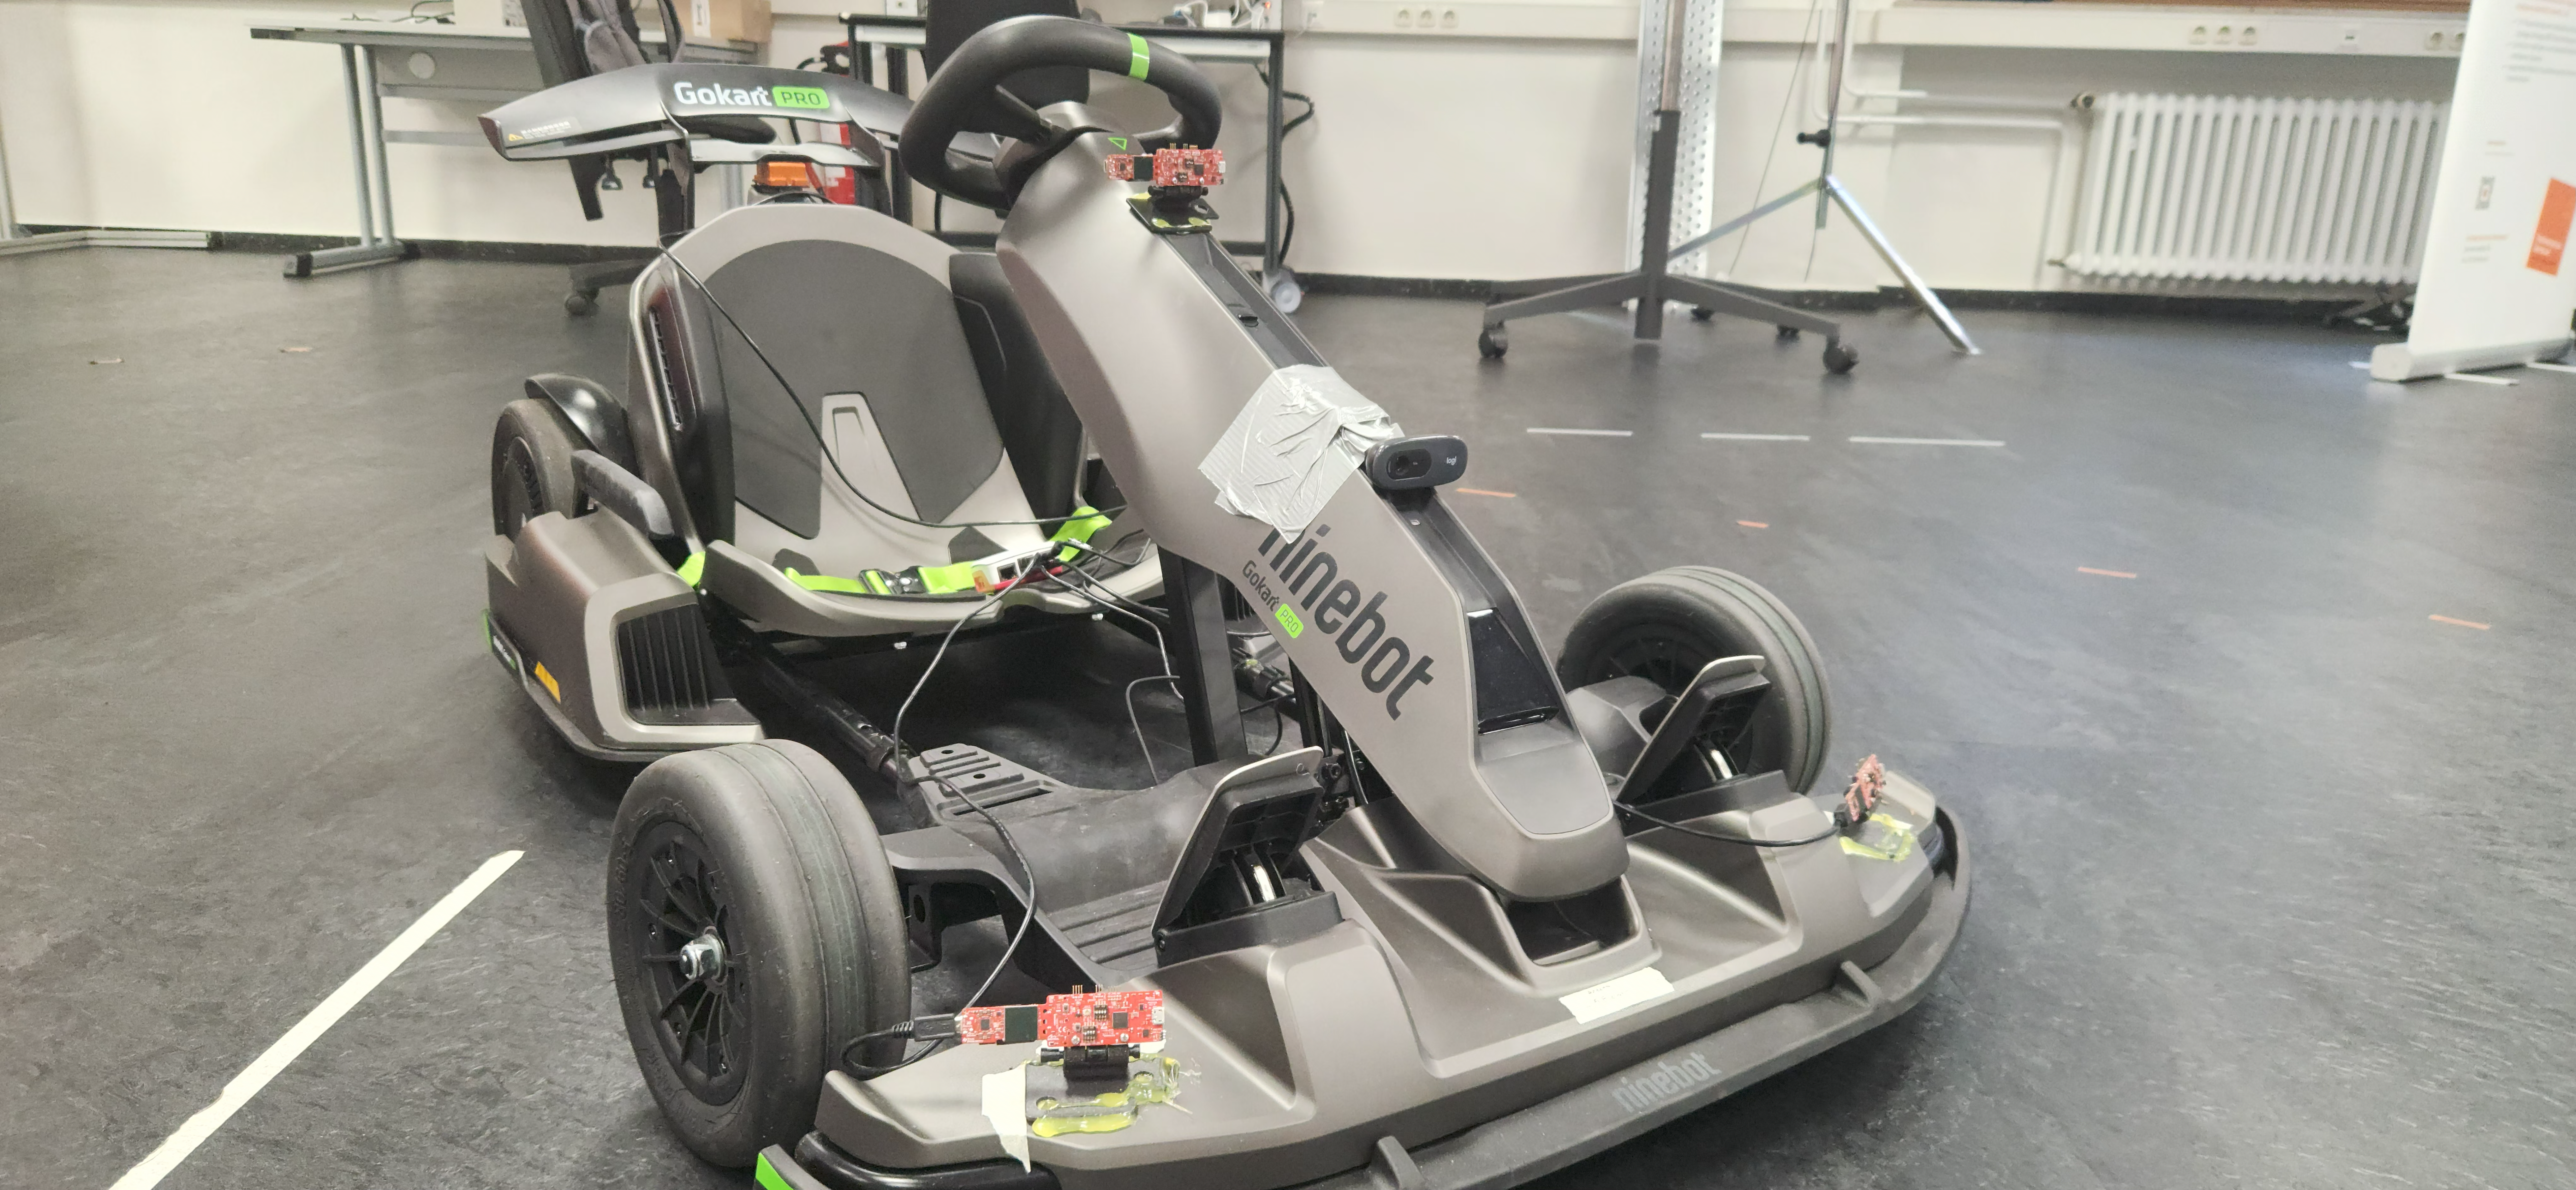
\includegraphics[width=\linewidth]{images/vehicleSystem.png}
        \caption{Ninebot test-vehicle system.}
        \label{fig:Ninebot_system}
    \end{subfigure}

    \vspace{1em} % vertical spacing between images

    \begin{subfigure}{0.9\linewidth}
        \centering
        \includegraphics[width=\linewidth]{images/vehicleSystemHighlight.png}
        \caption{Highlighted components of the Ninebot test-vehicle system.}
        \label{fig:Ninebot_system_highlight}
    \end{subfigure}

    \caption{Overview of the Ninebot test-vehicle system and highlighted components.}
    \label{fig:Ninebot_test-vehicle_System}
\end{figure}

Each item provide each own approach, contributions and implementation.
However not all of them are used for the actual solution, such is the case of the webcamera.
This component is used for the sole purpose of obtaining video material for later analysis.

\begin{comment}
    [25/09/2025]
    Check if this section shall be deleted or integrated with final result.
    As for integration is not such a great idea to implement a summarize of the project here.
    Only a brief introduction of the project shall discussed here.
    Contributions can be kept. As they are the whole intention of what it is accomplished here.
\end{comment}

To address the challenge posed by the sparsity and noise inherent in data obtained from mmWave sensors, a combination of techniques is proposed and organized into an easy-to-understand pipeline.
The workflow relies heavily on leveraging the Doppler effect and iterative closest point (ICP) alignment between submaps of frames to obtain more accurate motion information.

Instead of applying ICP globally, the key insight of this work is to track multiple clusters frame by frame, performing ICP iteratively on the aggregated submap and tracked clusters.
By doing so, the sparsity of radar data is mitigated, and the robustness of odometry estimation is improved.
This approach enhances stability and accuracy by focusing on the targets that are considered static in the environment and using them as references for ego-motion estimation.
This design choice aligns with recent findings showing that radar-driven odometry can achieve competitive performance, particularly when combined with Doppler velocity information \cite{EgoMotion_DopplerRadar, HighSpeed_Estimation}.

The full pipeline includes a RANSAC-based Doppler filter to remove dynamic points by assuming that the majority of detected reflections originate from static objects.
Any reflection from a dynamic object or target will typically exhibit a Doppler velocity that deviates from the fitted curve model provided by RANSAC, making it identifiable as an outlier.

The contributions of this work can be summarized as follows:  
\begin{enumerate}
    \item A radar ego-motion pipeline using mmWave sensors and an IMU for rotation, minimizing the hardware cost and system complexity.
    \item Integration of Doppler velocity and RANSAC filtering improves the distinction between static and dynamic objects.
    \item Submap aggregation to mitigate point cloud sparsity and improve alignment stability.
    \item Object tracking via clusters to identify and filter dynamic objects from the ego-motion estimation.
    \item Experimental validation using real-world data collected from a vehicle-mounted mmWave radar sensor.  
\end{enumerate}



